\chapter{Back to Basics}
\label{chapter:back_to_basics}

Psychologists distinguish between two categories of concepts or abilities related to the knowledge of concepts, depending on their level of abstraction. As Pepperberg puts it in \textit{The Alex Studies} about the parrot Alex \cite[p.52]{pepperberg1999alex}:

\blockquote{I needed to determine if [Alex] could respond not only to specific properties or patterns of stimuli, like pigeons who respond to positive instances of ``tree'', but also to classes or categories to which these specific properties or patterns belong. Could he, for example, go beyond recognizing what is or is not ``green'' to recognize the nature of the \textit{relationship} between a green pen and a blade of grass? In parlance of psychologists, the former ability (recognizing ``greenness'') is called \textbf{stimulus generalization}; the latter (recognizing the category ``color'') is called \textbf{categorical class formation}. The differences between these abilities are both subtle and important [\dots]. The extent to which most animals form categorical classes as defined above is as yet unknown.}

We added the bold text to show the important ideas.

This idea can as well be applied to machines and humans, not only to animals. Separating these two kind of concepts can be important, as categorical class formation requires a superior level of abstraction. However, in our studies we focus on the stimulus generalization, as it is already a challenge in itself.

\section{How can we know a concept has been learned?}
\label{sec:learned}

This is a very broad question, and applies not only to machine learning algorithms or artificial intelligent agents, but also to humans and animals. Of special interest is the case of Alex the parrot, whose knowledge was extensively studied. The only way to evaluate if he knew certain concepts was for him to correctly complete tasks that required the knowledge of those concepts.
Similarly, we need a general way of measuring knowledge that does not depend on the specific configuration of the features (which would be like studying the activations of the parrot’s brain), since finding some meaningful explanation in the feature distribution would be a sufficient condition to prove some knowledge, but not a necessary one. Also, it would be very difficult to compare different methods. Thus, we have to evaluate how the networks solve some basic tasks, like Alex did. 
To work with this problem, we resort to a simpler and more controlled dataset, the CLEVR dataset, that has a strong relation to Alex the parrot, as the attributes learned are exactly the same (color, material, shape and size).
To understand how we created the dataset, we can use an analogy with another famous animal, Clever Hans, a horse. Clever Hans seemingly understood the meaning of numbers, so when he was told a number by its owner, he tapped the floor that number of times (and was also capable of performing other similar tasks). However, what he was learning was to react to his owner’s body tension, and thus, he was giving the right answer for the wrong reasons: he didn’t know the actual concepts.
Neural networks can have a similar behaviour. They can learn concepts for a certain distribution (even generalizing correctly to unseen samples), but failing when the distribution changes, even when the concepts are the same. Because they do not really know the concept, they just learn to generate some useful “tailored-to-a-distribution” features (and they are very good at it).
To test this behaviour, we created a new version of CLEVR, that we name CLEVRA (CLEVR-Augmented), in which we add more possibilities to the already defined attributes (color, shape, size, material). This way, we have more options and we can create two different distributions of images, in which each distribution contains all the possible attributes, but their combinations are different. This is, if a distribution contains red balls, the other does not (it however will have red objects and other color balls, so the present concepts are the same).  We then create a train set from distribution 1, a test set from distribution 1 (testset-same) and a test set from distribution 2 (testset-different).
Concepts can be divided in two families depending on their hierarchy
As we said, we do not want to rely on the specific feature representation to evaluate what the network learned, so we came up with two different but similar ways of evaluating whether individual concepts have been learned:
Eval 1: we have a test dataset (not seen during training) with original images, a description of these images, and hard semantic negatives, which are images in which only a single attribute of a single object changes. Then, the network has to match the caption to the correct image, with 50% chance.
Eval 2: following the idea in Alain and Bengio (2016), we can measure the disentanglement of concepts in a certain layer of a neural network by training a simple linear classifier to classify the presence or absence of that concept given a set of features. If the linear classifier is capable of solving the problem, it means the features clearly.
We would like the network to do well in two different aspects:
Criteria 1: Performance in the evaluations, for both testset-same and testset-different
Criteria 2: Gap between testset-same and testset-different. If a method increases the performance of the two test sets from, say, 65% and 55% to 95% and 60% respectively, maybe it is better learning the concepts (Criteria 1 OK), but not in a really profound (generalizable) way, because the gap between the two distributions increases a lot (Criteria 2 KO)


\section{Our approach: semantic negatives and auxiliary tasks}

While choosing the right architecture for each task is very important in deep learning, we do not want to specifically tailor the architecture to the CLEVRA dataset or to the Eval tasks, because the idea of the project is to find ways for the system to find and extract more concepts in a general setting.

La gracia es que hem de pensar una nova tasca en train. Aixo en general correspon a una nova loss function (coloration, determinar si esta flipped o no…). Com diu AT, quins jocs hem de fer que la xarxa jugui perque reconegui “color” per separat, no “color+shape”. Isolate

\subsection{Hard semantic negatives}

Tema transformacions: Podem aplicar-les tambe a audio, pero hem de tenir en compte que no sempre sera tan facil com generar-lo. Ell pensa mes aviat en mechanical turk. 
Aleshores hi ha dos tipus de transformacions. 1) les externes i controlades/pensades per nosaltres, que serien per exemple donar imatges en blanc i negre a l’anotardor, i que les expliqui (obviament no parlara de colors), i 2) Les que es referia ell al principi, que es partint de una imatge (o audio), anem a destruir informacio, per exemple informacio de color, de mida (alterant aleatoriament les mides dels objectes), de posicio (segmentant la imatge amb algoritme de segmentacio i movent objectes de lloc), o fent random crops i canviant-los de posicio… (sempre randomly, res deterministic que les xarxes ho pillen molt facil). Tambe es pot fer algo semblant amb audio. La gracia es que si ens carreguem algo que la senyal d’audio pot reconstruir (i per tant algo significatiu, algun concepte o relacio) podrem explotar el poder de la relacio audio-imatge.
La historia que hem d’explicar es que els sistemes d’avui en dia van be pero no funcionen per a entendre atributs concrets, que no els aprenen, segurament perque no ho necessiten per a la tasca concreta. Per tant, si volem que les xarxes aprenguin be, hem de posar-los mes problemes, mes dificultats: semantic negative mining, combinat amb tasques que treballin els atributs

To try to force the network to learn concepts, we work with hard semantic negatives, this is, negative images in which the information associated to a certain concept has changed. This way, the network has to specifically focus on learning that concept. In order to generate hard semantic negatives, we have different options:
Render hard negatives
Generate negatives from input image
Black and white, and warping
Generated with GANs. They are generated from a segmentation mask containing the attributes. Some examples: [Segmentation mask | Generated image | Real ]


Examples of semantic negatives:
Original image
Black and white
Random warping



Generated (GAN) negative
(change red to yellow)
Rendered hard negative (change brown to blue)






For the case of GANs (and similarly for the other cases), the model would be something like:

Rendering hard negatives is only possible for a synthetic dataset such as CLEVRA, but they are very useful to gain insights into this approach. 
In a normal training, without negatives, we use the triplet loss, which is:
\begin{equation}
    L_{original} = \sum_i{\max{(0, \alpha + S(f_{im_i}, f_{au_}))}}
\end{equation}
Loriginal=imax0,+simfim(i), fau(i)-simfim(i), fau(ji) +imax0,+simfim(i), fau(i)-simfim(ji), fau(i), 
where  fau(i) and fim(i)represent the features for the audio and image i, $S(x,y)$ is a similarity function, the and $\alpha$ is a margin. It basically tries to get the corresponding features (from the same pair audio-image) close, while keeping the others far in the distance space defined by the similarity sim. The imposter j is sampled randomly.
When training with hard rendered negatives, we use these as negatives, along with the original loss, so we use the loss function:
Lhard neg=Loriginal+imax0,+simfim(i), fau(i)-simfim neg(i), fau(i). 
When using hard negatives generated from the input image, we add another element which consists in adding another triplet loss in which the hard negative is the positive image, and the randomly sampled image is the negative. This is to prevent the network from detecting that a hard negative is never the positive (for example, clearly a black and white image is not an image from the input distribution), and putting its representation always to zero. This is, we need to get a representation such that:
simfau(i), fim(i)>simfau(i), fim neg(i)>simfau(i), fim(ji)instead of simfau(i), fim(i)>simfau(i), fim(ji)>>simfau(i), fim neg(i)
This way, the loss is:
Ltriple-triplet=Lhard neg+imax0,+simfim neg(i), fau(i)-simfim(ji), fau(i) 
Notice how the margin  is not necessarily the same as the previous  one. This is because a large margin can lead to the network to give too much positive importance to the hard negative. A =0 would more or less lead to 
simfau(i), fim(i)>simfau(i), fim neg(i)simfau(i), fim(ji).


\begin{table*}\centering
\ra{1.3}
\begin{tabular}{@{}cccc@{}}\toprule
& Big & Green & Sphere \\
Normal training &
    \begin{minipage}{.2\textwidth}
      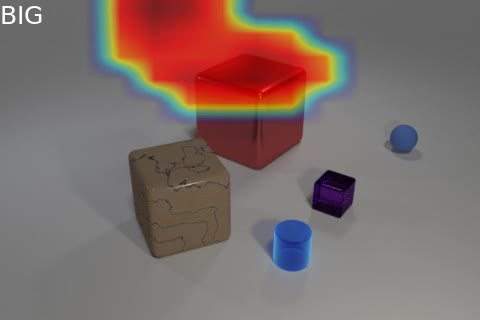
\includegraphics[width=\linewidth]{figures/CLEVR_activations/big_normal01.jpg}
    \end{minipage}
    &
    \begin{minipage}{.2\textwidth}
      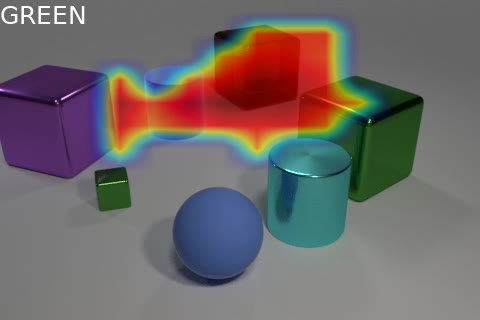
\includegraphics[width=\linewidth]{figures/CLEVR_activations/green_normal1.jpg}
    \end{minipage}
    &
    \begin{minipage}{.2\textwidth}
      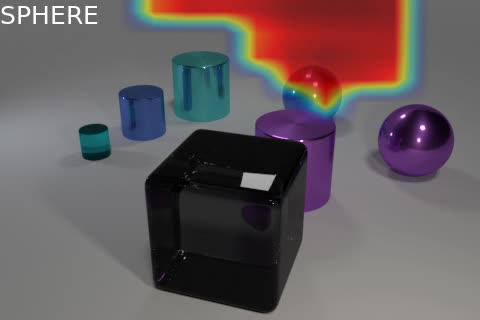
\includegraphics[width=\linewidth]{figures/CLEVR_activations/sphere_normal.jpg}
    \end{minipage}
\\ \\
All negatives &
    \begin{minipage}{.2\textwidth}
      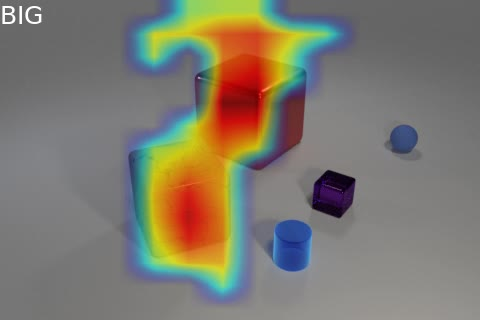
\includegraphics[width=\linewidth]{figures/CLEVR_activations/big_negimage01.jpg}
    \end{minipage}
    &
    \begin{minipage}{.2\textwidth}
      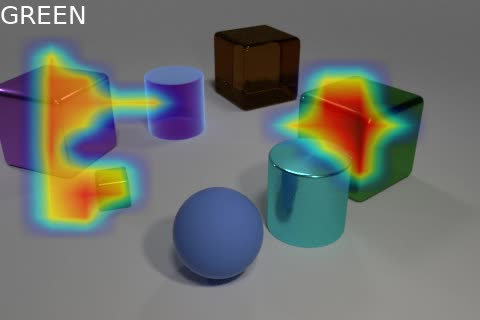
\includegraphics[width=\linewidth]{figures/CLEVR_activations/green_negimage01.jpg}
    \end{minipage}
    &
    \begin{minipage}{.2\textwidth}
      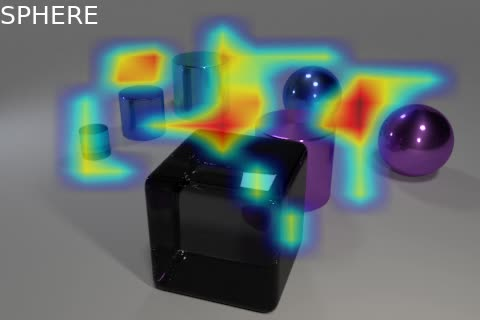
\includegraphics[width=\linewidth]{figures/CLEVR_activations/sphere_negimage01.jpg}
    \end{minipage}
\\ \\
\makecell{Other attribute \\ negatives} &
    \begin{minipage}{.2\textwidth}
      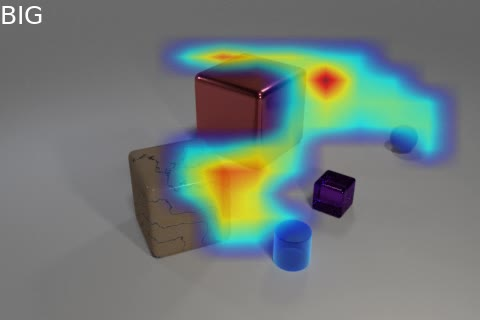
\includegraphics[width=\linewidth]{figures/CLEVR_activations/big_shape01.jpg}
    \end{minipage}
    &
        \begin{minipage}{.2\textwidth}
      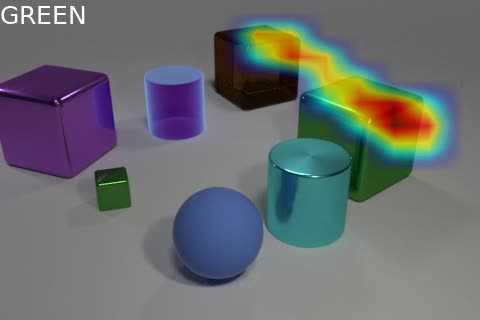
\includegraphics[width=\linewidth]{figures/CLEVR_activations/green_shape1.jpg}
    \end{minipage}
    &
    \begin{minipage}{.2\textwidth}
      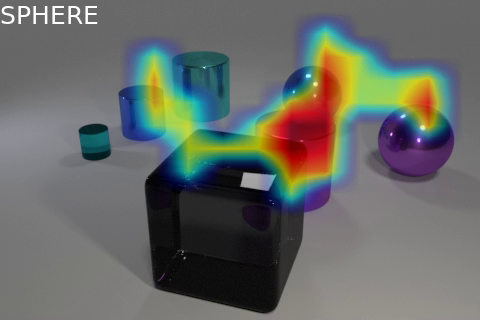
\includegraphics[width=\linewidth]{figures/CLEVR_activations/sphere_color.png}
    \end{minipage}
\\ \\
\makecell{Specific attribute \\ negatives} &
    \begin{minipage}{.2\textwidth}
      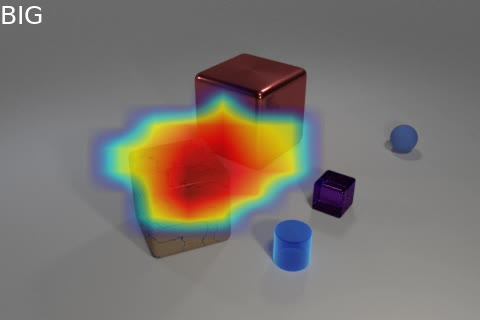
\includegraphics[width=\linewidth]{figures/CLEVR_activations/big_size01.jpg}
    \end{minipage}
    &
    \begin{minipage}{.2\textwidth}
      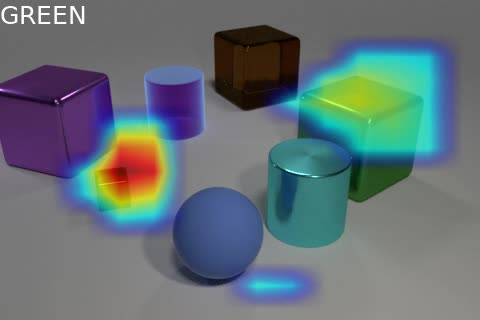
\includegraphics[width=\linewidth]{figures/CLEVR_activations/green_color01.jpg}
    \end{minipage}
    &
    \begin{minipage}{.2\textwidth}
      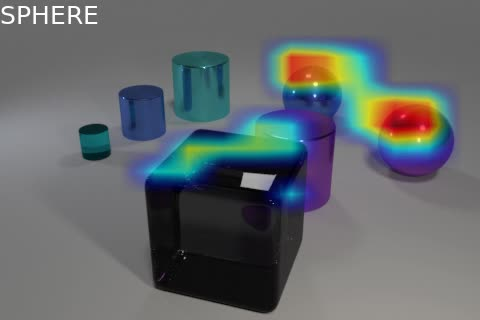
\includegraphics[width=\linewidth]{figures/CLEVR_activations/sphere_shape01.jpg}
    \end{minipage}
\\


\bottomrule
\end{tabular}
\caption[Caption]{Caption}
\end{table*}

\subsection{Reconstruction task}
Also, we argue that if we want the network to generalize and not just fit a single distribution, it may be useful to force it to do well on auxiliary tasks, and thus force it to find more meaningful representations. This is why we add a reconstruction task, in which we add a small network after the final features, and ask it to reconstruct the spatial information using the pooled information of the image, and the audio (text) information. Hopefully, this forces the representations to contain useful spatial and size information, and in general contain a more meaningful representation of the concepts.
Reconstructing the original image from the features using a conditional GAN would be very insightful, but unluckily, GAN state of the art is not there yet. 
Results and interpretation
A selection of results for Eval 1 is shown in the following table (we are still evaluating Eval 2). Other networks for the reconstruction have been used, as well as different kinds of rendered hard negatives (just color, just shape…), and combinations of methods, but the results in the table provide a general overview. Purple means testset-same, and blue means testset-different.

Eval 1 concept
Normal training
With rendered negatives
Reconstruction
Warping negatives
Black and white negatives (with = )
Color
0.81
0.69
0.92
0.70
0.69
0.70
0.60
0.70
0.49
0.50
Material
0.62
0.55
0.93
0.57
0.61
0.62
0.77
0.74
0.64
0.57
Shape
0.56
0.54
0.65
0.63
0.59
0.54
0.57
0.52
0.64
0.52
Size
0.81
0..66
0.90
0.79
0.87
0.64
0.89
0.64
0.90
0.80
Relation
0.52
0.54
0.86
0.71
0.77
0.66
0.52
0.50
0.81
0.63
Mean
0.66
0.60
0.85
0.68
0.71
0.63
0.67
0.62
0.70
0.59
Recall@5
0.99
0.09
0.97
0.10
0.93
0.19
0.91
0.10
0.83
0.13

Interpretation of the results:
Using rendered hard negatives improves a lot the criterion 1, even in the testset-different dataset. This means that the semantic negative idea works (which was something to be expected, because the network is trained to do well in this task). However, it creates a huge gap between distributions (bad criterion 2).
Using reconstruction improves criterion 2.
Combining the two previous points would seem a good idea to improve both criterion 1 and 2, but the results are that criterion 1 is even better than just with with hard negatives, but the gap instead of closing, increases. We still have to understand why.
Also, we did several studies on the relationship and correlation between the results in the two distributions (to see if when the test-same increases, the test-different increases), and also the correlation between Eval 1 and Recall. But none of these studies show a clear pattern or behaviour.
Checking the evolution of the test recall curves during training, the network is not overfitting to the distribution 1, because the train-different recall never goes down. 
Ongoing experiments with different margins (< ) are showing different results, so that can be a possible direction to understand how the network is working. We are working on that.

\section{Model Architecture}

For the CLEVR datset, we used the same architecture described in the Chapter ~\ref{chapter:starting_point}. However, we added two main changes:
\begin{enumerate}
    \item When working with \textbf{audio}, we 
\end{enumerate}

Tambe totes les arquitectures de FILM, reconstruction network...

\section{Datasets}



\label{sec:datasets}

\begin{table}[h]
\begin{tabular}{lll}
\textbf{Attribute} & \textbf{Number of options} & \textbf{Options}
\\ Shape    & 3 & Cube, Sphere, Cylinder 
\\ Color    & 8 & Cyan, Yellow, Red, Green, Blue, Gray, Brown, Purple 
\\ Size     & 2 & Large, Small 
\\ Material & 2 & Rubber, Metal  
\end{tabular}
\end{table}

Summary of all datasets created:

Comencem amb el CLEVR normal. Com tenim les scenes, creem diferents datasets de text (justificar cadascun):
- description data: tots els atributs de tots els objectes
- difficult data: locura "there are few red things ...". 
- only shape data
- only shape and color data
- sparse attributes. Alguns falten a vegades
- relation data. Incorporar "to the left of", no tot frases sueltas

Creem CLEVRA, que simplement es el CLEVR pero amb NEGATIUS. Implica per primer cop generar imatges noves. Aqui suposo que vaig generar tambe bastants estils de caption, pero al final ens hem quedat ja sempre amb la descripcio de tots, incloent relacions
- CLEVRA
\begin{table*}\centering
\ra{1.3}
\begin{tabular}{@{}ccccc@{}}\toprule
 \multicolumn{2}{c}{\textbf{Distribution A}} &&  \multicolumn{2}{c}{\textbf{Distribution B}} \\ 
 \cmidrule{1-2} \cmidrule{4-5}
Positives& Negatives & \phantom{ab} & Positives & Negatives\\
    \begin{minipage}{.2\textwidth}
      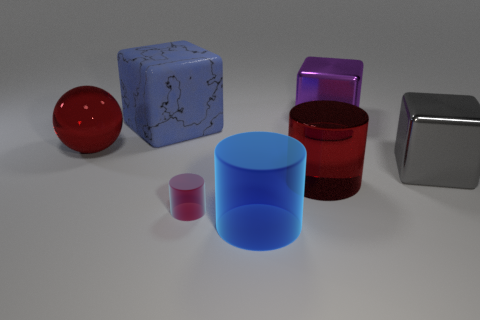
\includegraphics[width=\linewidth]{figures/clevr_datasets/CLEVRA_examples/train1.png}
    \end{minipage}
    &
    \begin{minipage}{.2\textwidth}
      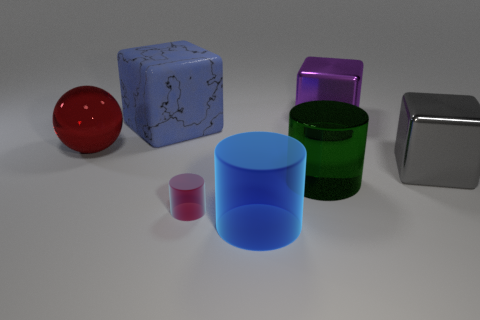
\includegraphics[width=\linewidth]{figures/clevr_datasets/CLEVRA_examples/train_color1.png}
    \end{minipage}
    &&
    \begin{minipage}{.2\textwidth}
      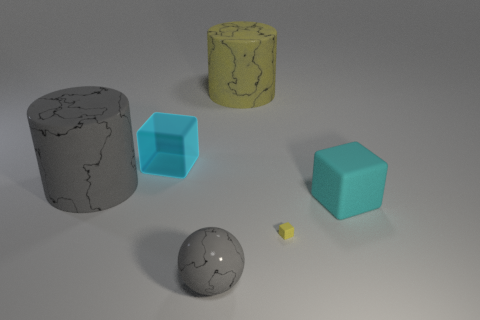
\includegraphics[width=\linewidth]{figures/clevr_datasets/CLEVRA_examples/test1.png}
    \end{minipage}
    &
        \begin{minipage}{.2\textwidth}
      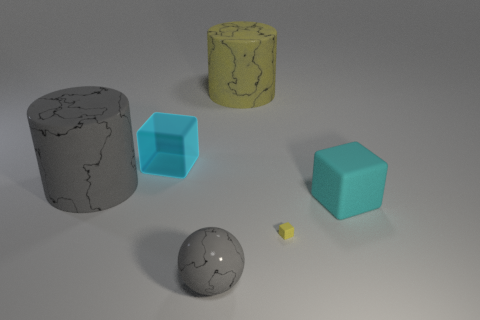
\includegraphics[width=\linewidth]{figures/clevr_datasets/CLEVRA_examples/test_color1.png}
    \end{minipage}
\\ \\
    \begin{minipage}{.2\textwidth}
      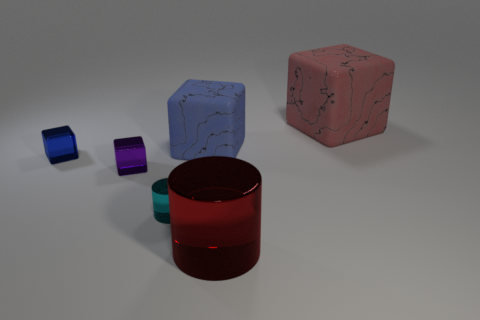
\includegraphics[width=\linewidth]{figures/clevr_datasets/CLEVRA_examples/train2.png}
    \end{minipage}
    &
    \begin{minipage}{.2\textwidth}
      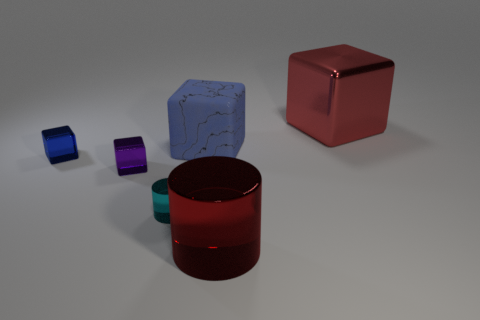
\includegraphics[width=\linewidth]{figures/clevr_datasets/CLEVRA_examples/train_material2.png}
    \end{minipage}
    &&
    \begin{minipage}{.2\textwidth}
      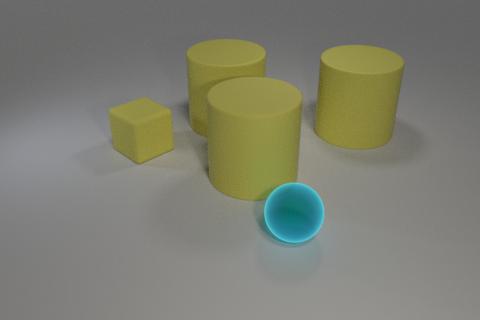
\includegraphics[width=\linewidth]{figures/clevr_datasets/CLEVRA_examples/test2.png}
    \end{minipage}
    &
        \begin{minipage}{.2\textwidth}
      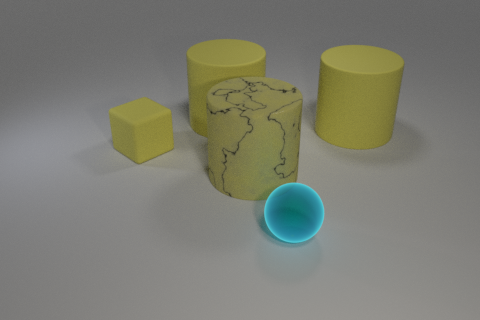
\includegraphics[width=\linewidth]{figures/clevr_datasets/CLEVRA_examples/test_material2.png}
    \end{minipage}
\\ \\
    \begin{minipage}{.2\textwidth}
      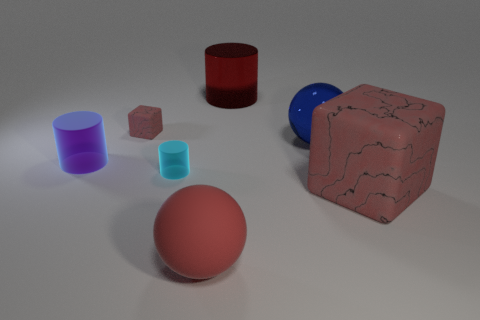
\includegraphics[width=\linewidth]{figures/clevr_datasets/CLEVRA_examples/train3.png}
    \end{minipage}
    &
    \begin{minipage}{.2\textwidth}
      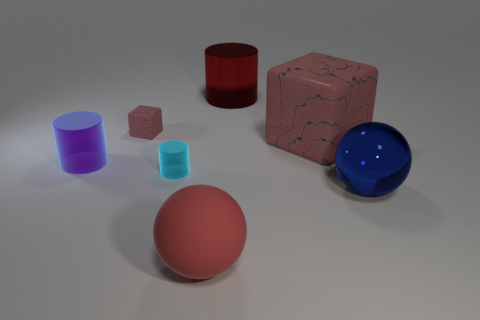
\includegraphics[width=\linewidth]{figures/clevr_datasets/CLEVRA_examples/train_relation3.png}
    \end{minipage}
    &&
    \begin{minipage}{.2\textwidth}
      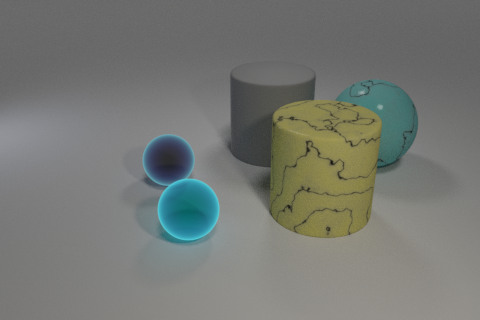
\includegraphics[width=\linewidth]{figures/clevr_datasets/CLEVRA_examples/test3.png}
    \end{minipage}
    &
        \begin{minipage}{.2\textwidth}
      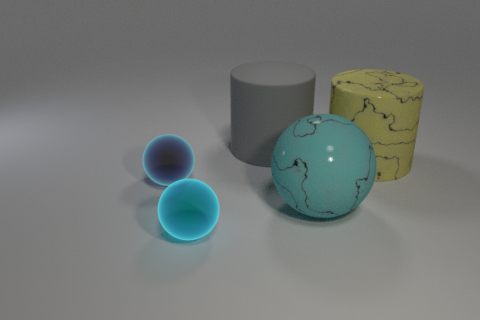
\includegraphics[width=\linewidth]{figures/clevr_datasets/CLEVRA_examples/test_relation3.png}
    \end{minipage}
\\ \\
    \begin{minipage}{.2\textwidth}
      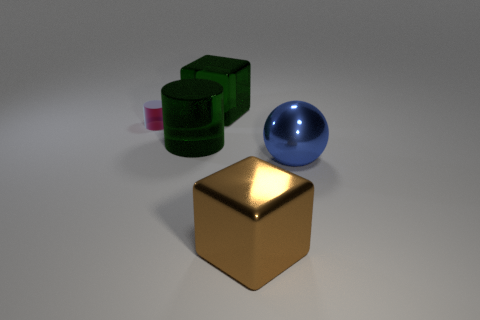
\includegraphics[width=\linewidth]{figures/clevr_datasets/CLEVRA_examples/train4.png}
    \end{minipage}
    &
    \begin{minipage}{.2\textwidth}
      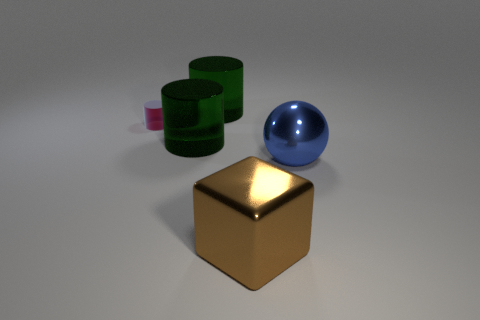
\includegraphics[width=\linewidth]{figures/clevr_datasets/CLEVRA_examples/train_shape4.png}
    \end{minipage}
    &&
    \begin{minipage}{.2\textwidth}
      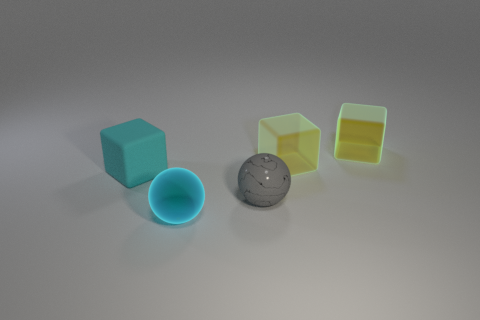
\includegraphics[width=\linewidth]{figures/clevr_datasets/CLEVRA_examples/test4.png}
    \end{minipage}
    &
        \begin{minipage}{.2\textwidth}
      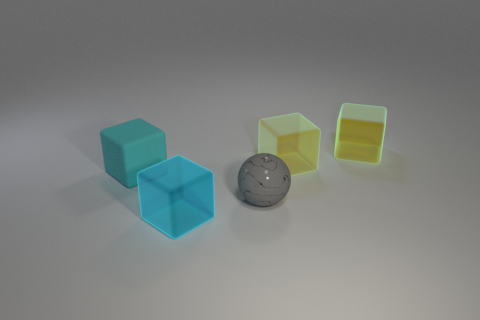
\includegraphics[width=\linewidth]{figures/clevr_datasets/CLEVRA_examples/test_shape4.png}
    \end{minipage}
\\ \\
    \begin{minipage}{.2\textwidth}
      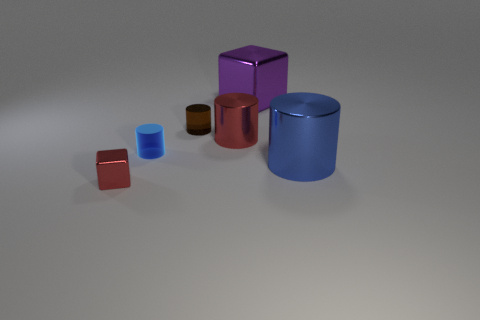
\includegraphics[width=\linewidth]{figures/clevr_datasets/CLEVRA_examples/train5.png}
    \end{minipage}
    &
    \begin{minipage}{.2\textwidth}
      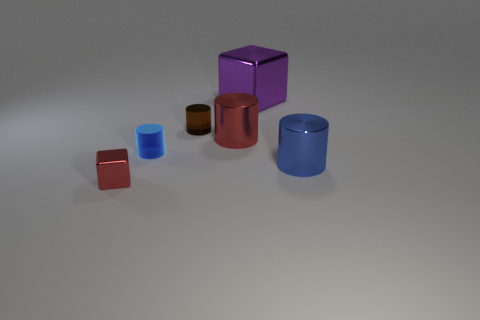
\includegraphics[width=\linewidth]{figures/clevr_datasets/CLEVRA_examples/train_size5.png}
    \end{minipage}
    &&
    \begin{minipage}{.2\textwidth}
      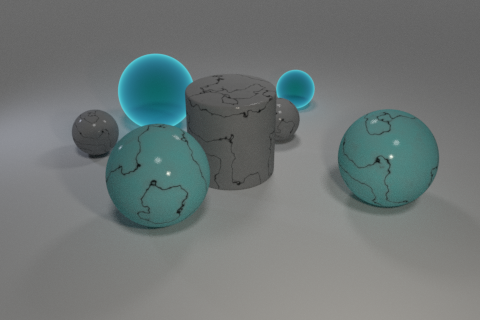
\includegraphics[width=\linewidth]{figures/clevr_datasets/CLEVRA_examples/test5.png}
    \end{minipage}
    &
        \begin{minipage}{.2\textwidth}
      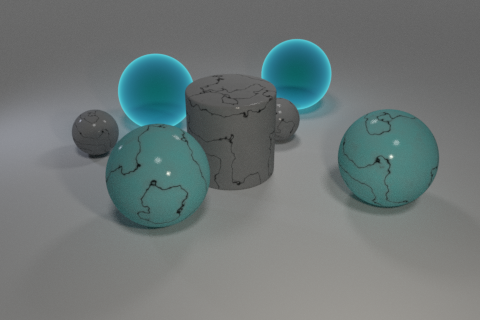
\includegraphics[width=\linewidth]{figures/clevr_datasets/CLEVRA_examples/test_size5.png}
    \end{minipage}
\\ 

\bottomrule
\end{tabular}
\caption[CLEVR\_B dataset examples]{CLEVR\_B dataset examples. There are five examples from each distribution, with corresponding negatives. Each row shows a different negative (color, material, relation, shape, size). There is a negative for each attribute and each image, so there are a total of six similar images for each example (positive and five negatives), though in this table we only show the positive and one of the negatives.}
\end{table*}


- CLEVRset. Ignorar


Despres vam veure que haviem de crear dues distribucions diferents, i per aixo ens vam posar a fer el SCLEVR, on generem mes tipus de materials i shapes.
Combinacions color + material vistes i no vistes en test:
Seen to no seen errors: 97/840 (11.57\%)
No seen to seen errors: 358/667 (53.67\%)

- SCLEVR
\begin{table*}\centering
\ra{1.3}
\begin{tabular}{@{}ccc@{}}\toprule
&\textbf{Example 1}&\\
\midrule
Positive & Negative Color & Negative Material \\
    \begin{minipage}{.3\textwidth}
      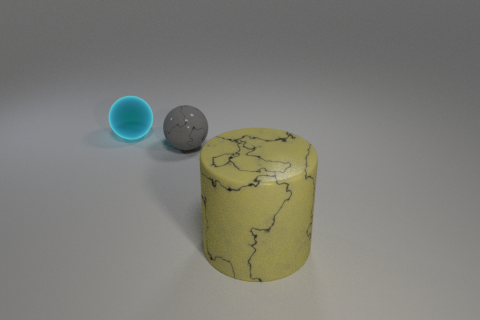
\includegraphics[width=\linewidth]{figures/clevr_datasets/sclevr_ori1.png}
    \end{minipage}
    &
    \begin{minipage}{.3\textwidth}
      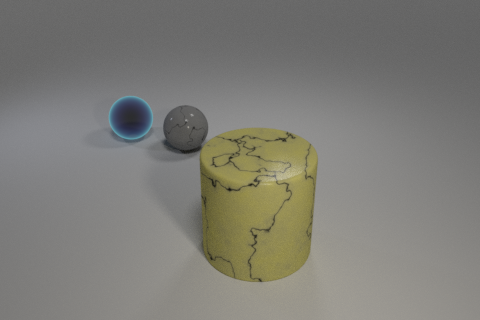
\includegraphics[width=\linewidth]{figures/clevr_datasets/sclevr_col1.png}
    \end{minipage}
    &
    \begin{minipage}{.3\textwidth}
      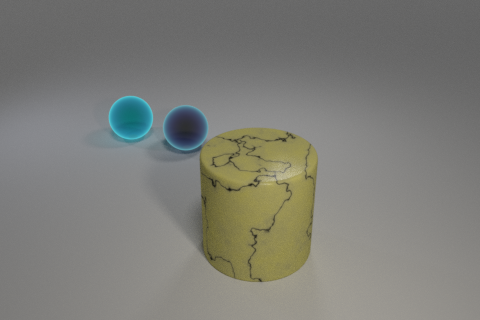
\includegraphics[width=\linewidth]{figures/clevr_datasets/sclevr_mat1.png}
    \end{minipage}
\\
Negative Shape & Negative Size & Negative Relation \\
    \begin{minipage}{.3\textwidth}
      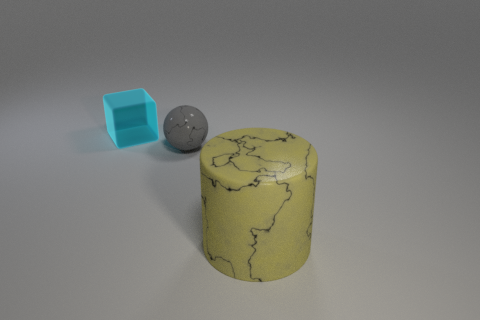
\includegraphics[width=\linewidth]{figures/clevr_datasets/sclevr_shape1.png}
    \end{minipage}
    &
    \begin{minipage}{.3\textwidth}
      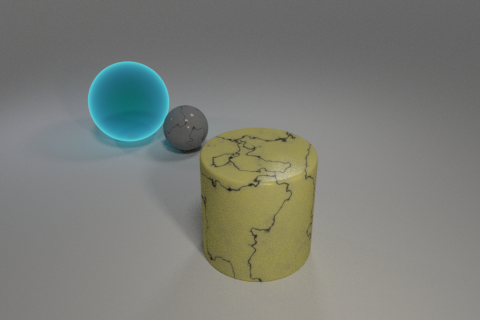
\includegraphics[width=\linewidth]{figures/clevr_datasets/sclevr_size1.png}
    \end{minipage}
    &
    \begin{minipage}{.3\textwidth}
      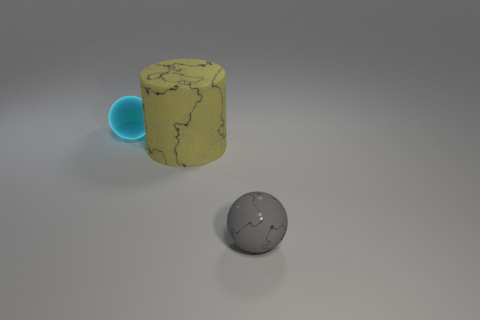
\includegraphics[width=\linewidth]{figures/clevr_datasets/sclevr_rel1.png}
    \end{minipage}
\\
\midrule
&\textbf{Example 2}& \\ \midrule
Positive & Negative Color & Negative Material \\
    \begin{minipage}{.3\textwidth}
      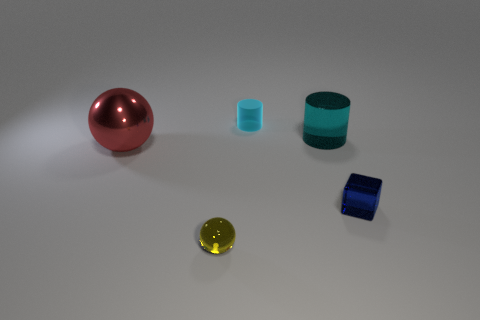
\includegraphics[width=\linewidth]{figures/clevr_datasets/sclevr_ori2.png}
    \end{minipage}
    &
    \begin{minipage}{.3\textwidth}
      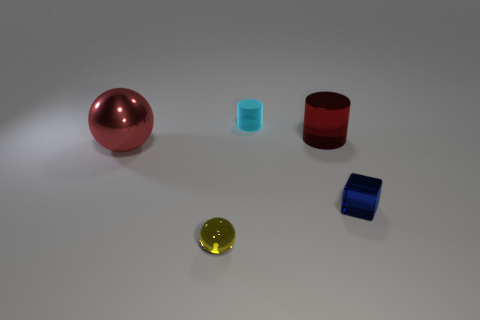
\includegraphics[width=\linewidth]{figures/clevr_datasets/sclevr_col2.png}
    \end{minipage}
    &
    \begin{minipage}{.3\textwidth}
      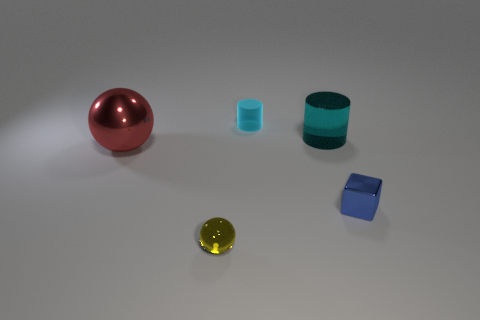
\includegraphics[width=\linewidth]{figures/clevr_datasets/sclevr_mat2.png}
    \end{minipage}
\\
Negative Shape & Negative Size & Negative Relation \\
    \begin{minipage}{.3\textwidth}
      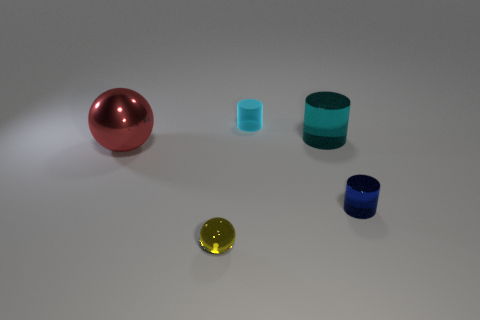
\includegraphics[width=\linewidth]{figures/clevr_datasets/sclevr_shape2.png}
    \end{minipage}
    &
    \begin{minipage}{.3\textwidth}
      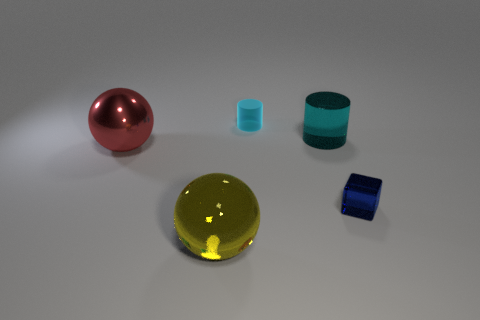
\includegraphics[width=\linewidth]{figures/clevr_datasets/sclevr_size2.png}
    \end{minipage}
    &
    \begin{minipage}{.3\textwidth}
      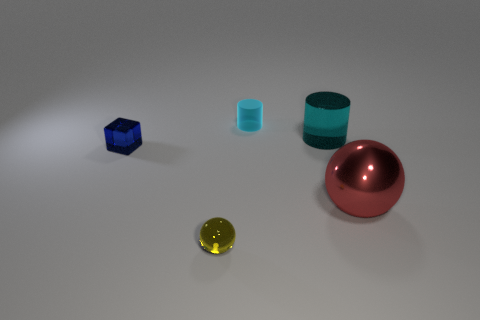
\includegraphics[width=\linewidth]{figures/clevr_datasets/sclevr_rel2.png}
    \end{minipage}
\\

\bottomrule
\end{tabular}
\caption{Caption}
\end{table*}


Veiem que encara hi ha una certa desproporcio en SCLEVR, Atributs secundaris que no son shape si els havia vist els considerava millors... Creem SCLEVR2, amb 20 colors i idealment mes simetria i tal. Pero QUIN ERA EL PROBLEMA?
- SCLEVR2

Aixi que creem SCLEVR3, amb 4 possibilitats per a cada atribut (nomes un size, per aixo)
- SCLEVR3

Desired  properties:  we  build  a  version  of  the  CLEVR  dataset  such  that:  
\begin{enumerate}
    \item Attributes:  There  are  4  materials,  4  shapes  and  4  colors.  \item Training  set  only  sees  half  of  the  combinations  of  triplets. \item Avoid  bias:  Training  set  sees  all  the  combinations  for  pairs  of  attributes  
    \item Evaluation  set:  It  has  pairs  of  images  (positive,  negative)  with  only  one  attribute  change  between  them.  
    \begin{enumerate}
        \item Test  set  A:  The  combination  of  (material,  shape,  color)  has  been  seen  in  training.  
        \item Test  set  B:  The  combination  of  (material,  shape,  color)  has  not  been  seen  in  training. 
    \end{enumerate}
\end{enumerate}


\begin{table*}\centering
\ra{1.3}
\begin{tabular}{@{}ccc@{}}\toprule
&\textbf{Positive}& \\
&
\begin{minipage}{.3\textwidth}
  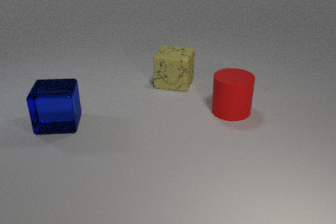
\includegraphics[width=\linewidth]{figures/clevr_datasets/SCLEVR3_original.png}
\end{minipage}
& \\
&\textbf{Negatives}& \\
\cmidrule{2-2}
Shape & Color & Material \\
    \begin{minipage}{.3\textwidth}
      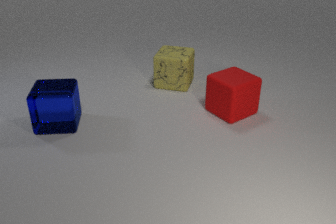
\includegraphics[width=\linewidth]{figures/clevr_datasets/SCLEVR3_negshape.png}
    \end{minipage}
    &
    \begin{minipage}{.3\textwidth}
      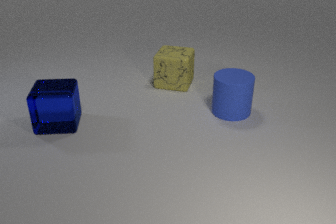
\includegraphics[width=\linewidth]{figures/clevr_datasets/SCLEVR3_negcolor.png}
    \end{minipage}
    &
    \begin{minipage}{.3\textwidth}
      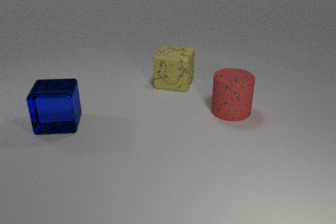
\includegraphics[width=\linewidth]{figures/clevr_datasets/SCLEVR3_negmat.png}
    \end{minipage}
\\
\bottomrule
\end{tabular}
\caption{Caption}
\end{table*}

\begin{table*}\centering
\begin{tabularx}{\linewidth}{c X}
  \toprule
  Caption & \hfill \textit{There is a red cylinder to the right of a yellow marble cube} \hfill\null \\
  \midrule
  Images & 
    \hfill \makecell{Option 1 (correct) \\ 
        \begin{minipage}{.3\textwidth}
          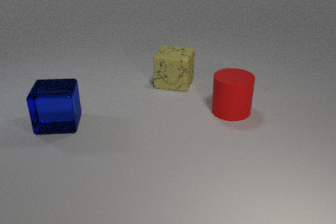
\includegraphics[width=\linewidth]{figures/clevr_datasets/SCLEVR3_original.png}
        \end{minipage} \\} 
    \hfill \makecell{Option 2 (incorrect) \\ 
        \begin{minipage}{.3\textwidth}
          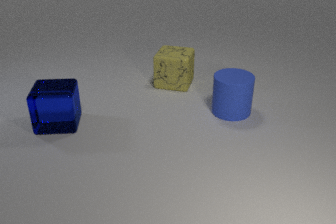
\includegraphics[width=\linewidth]{figures/clevr_datasets/SCLEVR3_negcolor.png}
        \end{minipage}} \\
  \bottomrule
\end{tabularx}
 \caption{Evaluation:  We  make  the  system  decide  between  two  images, which  are  exactly  the  same but  one  attribute  changes.  This  combination  of attributes+shape  has  never  been  seen  before  by  the  network }
\end{table*}

\begin{table*}\centering
\ra{1.3}
\begin{tabular}{@{}lccccccc@{}}\toprule
& \multicolumn{3}{c}{Test set A (seen attributes)} & \phantom{abc}& \multicolumn{3}{c}{Test set B (unseen attributes)} \\
\cmidrule{2-4} \cmidrule{6-8} 
& Color & Shape & Material && Color & Shape & Material \\ \midrule
Rendered negatives & 0.995 & 0.0.74 & 0.995 && 0.0.95 & 0.56 & 0.91\\
Stitched negatives & 0.997 & 0.60 & 0.88 && 0.97 & 0.56 & 0.80\\
Random negatives & 0.72 & 0.56 & 0.62 && 0.71 & 0.51 & 0.61\\
\bottomrule
\end{tabular}
\caption{Caption}
\end{table*}

Independentment als anteriors, per a fer certs estudis necessitem segmentacions. CLEVR normal amb segmentacions:
- CLEVRSEG

- halloween i clover?


\section{Visualizations}

As we said before, we cannot rely solely on feature representations to assess the learning of a concept (they can be a sufficient but not strictly necessary …). However, they are very useful to try to understand (“debug”) our system, and thus being able to improve it. 

- videos amb mapes de on es veu a que s'esta referint. Tant per a audio com a text (en CLEVR). Obviament tambe posar-ho per al projecte de ECCV (extra material o com es digui)

- Clustering experiments



- Tots els experiments de anar de gros a petit i tal. Ficar els experiments dins un context. En plan "volem veure quina part de la xarxa es dedica a quina cosa..."


\begin{wrapfigure}{R}{\textwidth}
\subfloat{\includegraphics[width=0.3\linewidth]{figures/change_size/image31.png}}
\hspace{2mm}
\subfloat{\includegraphics[width=0.3\linewidth]{figures/change_size/image28.png}}
\hspace{2mm}
\subfloat{\includegraphics[width=0.3\linewidth]{figures/change_size/image18.png}}
\\
\subfloat{\includegraphics[width=0.3\linewidth]{figures/change_size/image32.png}}
\hspace{2mm}
\subfloat{\includegraphics[width=0.3\linewidth]{figures/change_size/image19.png}}
\hspace{2mm}
\subfloat{\includegraphics[width=0.3\linewidth]{figures/change_size/image21.png}} 
\\
\subfloat{\includegraphics[width=0.3\linewidth]{figures/change_size/image27.png}}
\hspace{2mm}
\subfloat{\includegraphics[width=0.3\linewidth]{figures/change_size/image12.png}}
\hspace{2mm}
\subfloat{\includegraphics[width=0.3\linewidth]{figures/change_size/image22.png}}
\caption[Caption]{caption}
\label{fig:size_change}
\end{wrapfigure}

-Tambe he fet l’experiment de restar els matchmaps dels negatius i el positiu, i mirar les neurones que mes canviaven en positiu i negatiu. Si es miren (per als casos en que els matchmaps realment empitjora per al negatiu) les activacions de les neurones, es pot determinar facilment el color. Guay

Crec que aixo esta en un video

Afegir les imatges de CLEVR\_activations amb explicacio de que es cada cosa

Note on disentanglement: disentanglement is a very studied tal i qual (referencies). Disentanglement treball directament en fer disentanglement de features, tenir representacions separades en el latent space. Aixo es una manera que pot ser suficient per a aillar conceptes, pero nosaltres ho mirem des d'un punt molt mes global.